\documentclass{report} \usepackage[T1]{fontenc} \usepackage[italian]{babel}
\usepackage{color}
\usepackage[type={CC},modifier={by-sa},version={4.0},]{doclicense}
\usepackage{cite}

\usepackage{graphicx}
\graphicspath{ {./media/images/} }
\usepackage{float}

\usepackage{hyperref}

\title{Title} \author{Daniele Melocchi\\Agnese Montanaro\\Matteo
Savatteri}

\begin{document}
\maketitle
\setcounter{page}{2}

Copyright Daniele Melocchi, Agnese Montanaro, Matteo Savatteri -
\the\year \doclicenseThis \thispagestyle{empty}

\tableofcontents

\chapter{Introduzione}
Questo documento presenta un ciclo di lezioni svolte nella modalità
della didattica a distanza (\emph{DAD}) e
indirizzate ad una classe 1\textsuperscript{a} Liceo Scientifico,
riguardanti le basi della cinematica, il moto rettilineo uniforme
e uniformemente accelerato.

Il percorso didattico è suddiviso in tre moduli, all'interno dei quali
sono affrontati i seguenti argomenti, ordinati secondo un criterio
di complessità crescente, partendo da un approccio completamente
qualitativo, per passare ad uno via via più quantitativo:
\begin{enumerate}
\item Posizioni, istanti, distanze e intervalli temporali, leggi orarie.
\item Velocità media, velocità istantanea, moto rettilineo uniforme.
\item Accelerazione media, accelerazione istantanea, moto uniformemente
      accelerato.
\end{enumerate}

Il percorso si fonda sul \emph{modello didattico delle 5E}\cite{bybee2006bscs}.
Ogni modulo si suddivide dunque in cinque sezioni, nelle quali sono presentate
attività, riflessioni, suggerimenti e problematiche, per ciascuna delle
cinque fasi di questo metodo di natura \emph{inquiry}:
\emph{engage}, \emph{explore}, \emph{explain}, \emph{extend}, \emph{evaluate}.

\section{Propedeuticità}
Al fine della buona riuscita di questo percorso, è necessario che gli
studenti coinvolti abbiano affrontato e consolidato la comprensione
dei seguenti argomenti:
\begin{itemize}
\item Operazioni algebriche elementari (es. frazioni e potenze).
\item Equazioni di primo grado.
\item Rappresentazioni di numeri su un asse ordinato.
\item Rappresentazione di coppie di numeri (punti) su un diagramma
      cartesiano.
\item Conoscenza di unità di misura di grandezze fondamentali.
      (es. lunghezza, tempo)
\end{itemize}

\chapter{Posizioni, Istanti e intervalli}
Nel presente modulo lo studente familiarizza con i concetti
di posizione, distanza, istante (inteso come
\emph{lettura di orologio}) e intervallo di tempo.
Succesivamente, guidato dal docente, esplora le relazioni
che intercorrono tra queste grandezze nel contesto del moto di
un corpo, giungendo ad una comprensione qualitativa dei
concetti di \emph{evento} e \emph{legge oraria}.

\section{Engage}
\begin{itemize}
\item \textbf{Tempo richiesto:} 15 min.
\item \textbf{Materiale:} Computer
\end{itemize}

Il docente mostra agli studenti
\footnote{
Nel contesto della DAD, il docente può utilizzare
una piattaforma web di videotelefonia, che supporti la condivisione
di file multimediali. Jitsi Meet\textsuperscript{\textregistered},
Zoom\textsuperscript{\textregistered},
Google Meet\textsuperscript{\textregistered} e
Microsoft Teams\textsuperscript{\textregistered}
sono solo alcuni esempi.
}
il video di un fenomeno fisico riprodotto \emph{in reverse} (ovvero ribaltando
l'asse temporale). Il fenomeno fisico rappresentato dovrebbe essere scelto
in modo che sia difficile (o impossibile) distinguere se il video viene
riprodotto in reverse oppure no. Il moto di un pendolo semplice,
di un \emph{pendulum wave} o di altri moti periodici costituiscono buoni
esempi.

Nel contesto di questo progetto si è scelto il video in \emph{slow motion}
di un colibrì in volo, che si nutre da un tubicino (Figura \ref{fig:hummingbird}) 
\footnote{
\`E possibile scaricare il video presso
\href{https://github.com/savaroskij/PED1/blob/master/progetto_finale/media/video/Hummingbird.mp4?raw=true}{questa pagina web}
. L'indirizzo del video originale si trova nella bibliografia\cite{hbird}.
}
. Solamente la componente video, e non quella audio, è stata inverta per
aumentare l'effetto di inganno.

\begin{figure}
\centering
  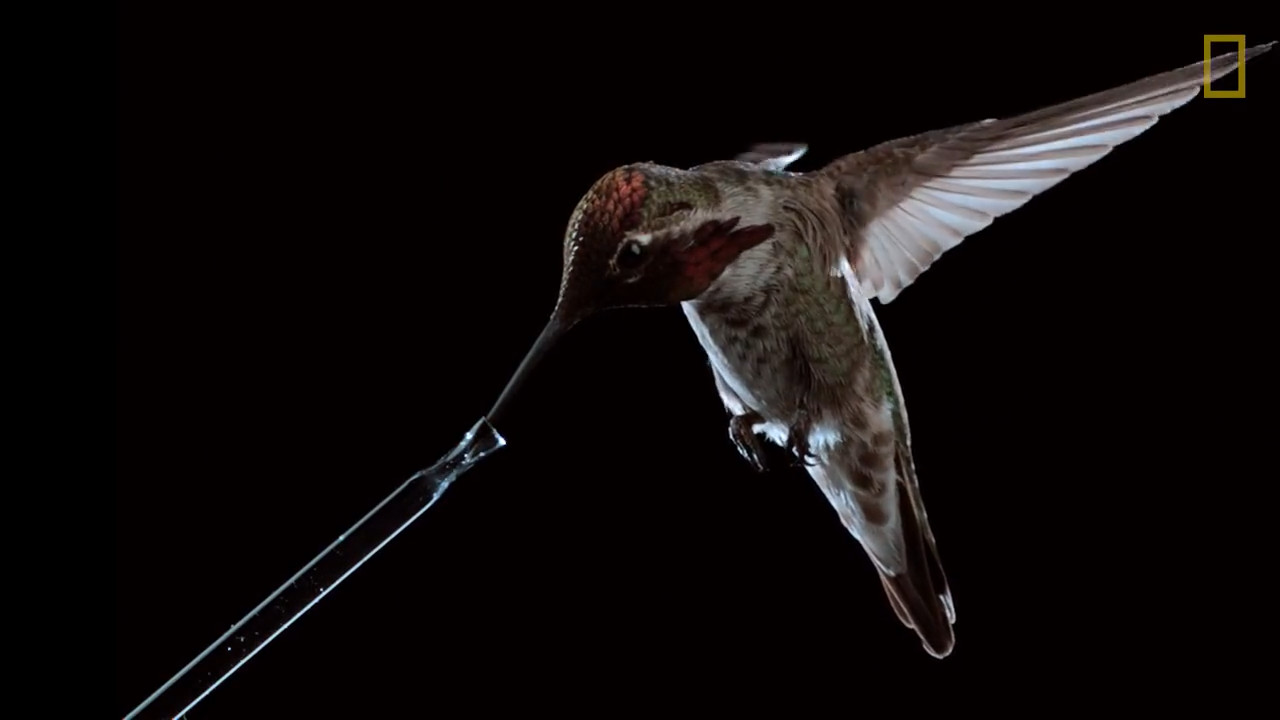
\includegraphics[width=\textwidth]{Hummingbird}
  \caption{Un frame del video di un colibrì in volo che si nutre da un tubicino.}
  \label{fig:hummingbird}
\end{figure}

Il docente in seguito chiede agli studenti di descrivere quanto viene
visualizzato, e solamente infine svela che il video è riprodotto in
reverse. In questo modo l'insegnante ha l'occasione di far notare
allo studente, e lo esplicita, che per studiare qualsiasi fenomeno fisico
occorrono chiari riferimenti spaziali e temporali.


\bibliography{bibliografia}{}
\bibliographystyle{plain}

\end{document}
